\section{Results and Discussion}
\label{sec:ResDisc}
To demonstrate the quality of JFUSE, we used both real and synthetic JSON collections in our experiments. First, we specified the environment in which the experiments took place, and then, we presented both real and synthetic experiment results.

Based on the definitions mentioned in Section~\ref{sec:SchDisc}, our approach was developed using the C++ programming language. 
It can be found  at \textit{https://github.com/NathyBanhara/JFUSE}. 
The experiments were performed on a server machine with four Intel(R) Xeon(R) CPU E7- 4850 (2.00GHz) and 128 GB RAM, running a Linux 4.15.0-50 kernel (Ubuntu 18.04.2 LTS distribution).  
We ran an empirical experiment on various datasets and studied some JSON collections to find the suitable values for all the thresholds, and they are: 
\(Thr_m \geq 0.9\) , 
\(Thr_t \geq 0.5\), 
\(Thr_{str} \leq 20\), 
%\(Thr_{int} \leq 100\), 
\(Thr_{arr} \geq 0.9\), 
\(Thr_{obj} \leq 0.1\), and 
\(Thr_{dt} \geq 0.7\).


\subsection{Real Data Experiments}
Two JSON document collections were used to test our tool with real data.  
The first one was taken from \citep{Sp+21}. The study case refers to pharmaceutical data (\textit{PHC}), which allows testing on scenarios such as objects as collections and enumeration detection, besides basic types. 
The other one regards Russia's 2018 election tweets user activity (TWC). Obtained from Kaggle\footnote{https://www.kaggle.com/datasets/borisch/russian-election-2018-twitter}, the dataset contains tweet records and it is interesting due to its many optional fields. 
We ran the experiments five times to ensure that there would be no discrepancy in the execution time, and it was verified since the standard deviation was less than 1\%. We reported the execution time average. 

%
As Table~\ref{tab:ComparaReal} shows, with a size of 165Mb and 7,226,980 keys, the pharmaceutical experiments had an average performance time of 1m59.947s. The TWC schema, a much larger collection with 11,5GB and 420,022,871 keys, was generated after about 110m46.484s. 
Regarding the collection size, TWC is 8.7 times bigger than PHC, having 58 times more keys than PHC. 
However, concerning the execution time, TWC was 69 times slower than PHC. 
We believe that the number of keys impacts the computational performance more than the size of collections, and because of that, we believe that our approach scales well when facing huge collections. 
Moreover, the column \textit{Schema Keys} shows the number of keys in the resulting schema: PHC comprises 11 keys and TWC has 210 keys. It shows that the built schemas are concise.

% twitter 8.7 times bigger than pharmaceutic 
% twitter 58 times than pharmaceutic (# of keys)
% Performance 69 times slower than pharmaceutic


\begin{table}[!hbt]
\centering
\small
\caption{Table showing the results obtained from experiments with real data.}
\begin{tabular}{|l|r|r|r|r|}
\hline
\textbf{Collection} & \textbf{Size} & \textbf{Keys} & \textbf{Time (s)} & \textbf{Keys} \\ \hline
Pharmaceutic        & 165Mb         & 7,226,980     & 1m59.947s   & 11      \\ \hline
Twitter             & 11,5GB        & 420,022,871   & 110m46.484s & 210    \\ \hline
\end{tabular}
\label{tab:ComparaReal}
\end{table}

In the following, we present the schema extracted from PHC (based on the meta-model described in Section~\ref{sec:SchDisc}).


\noindent
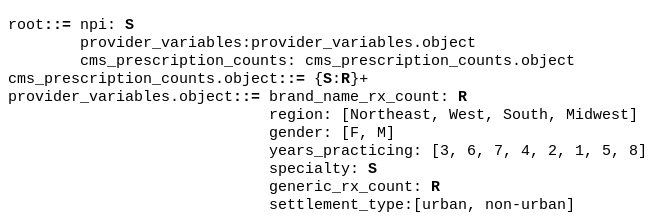
\includegraphics[scale=.6]{Figures/PharmSchema.png}

% \noindent
% \textit{root}::= \textbf{npi:} $\mathbb{S}$ \textbf{provider\_variables:} \textit{provider\_variables.object} \\
% \hspace*{1.2cm} \textbf{cms\_prescription\_counts:} \textit{cms\_prescription\_counts.object}\\
% \textit{cms\_prescription\_counts.object}::= \{($\mathbb{S}$ : $\mathbb{R}$)$^+$\}\\
% \textit{provider\_variables.object}::= \textbf{brand\_name\_rx\_count:} $\mathbb{R}$ \\
% \hspace*{1cm}\textbf{region:} [Northeast, West, South, Midwest] \textbf{gender:} \textit{[F, M]} \\
% \hspace*{1cm}\textbf{years\_practicing:} \textit{[3, 6, 7, 4, 2, 1, 5, 8]} \textbf{specialty:} $\mathbb{S}$ \textbf{generic\_rx\_count:} $\mathbb{R}$ \\
% \hspace*{1cm}\textbf{settlement\_type:} \textit{[urban, non-urban]}

As can be seen, \texttt{cms\_prescription\_counts.object} represents an object as collection, and the metadata inside it is represented as data, which means the optional fields in \texttt{cms\_prescription\_counts.object} are greater than $Thr_{dt}$.  
On the other hand, \texttt{region.string}, \texttt{gender.string}, \texttt{years\_practicing.integer}, and \texttt{settlement\_type.string} are all enumerations.

\subsection{Synthetic Experiments}
We built five new synthetic collections from the Figure~\ref{fig:JSONEx} template to produce collections containing every type that JFUSE intends to discover (\textit{i.e.}, atomic types, tagged unions, metadata, objects as collections, arrays as tuples, and enumeration). 
We ran the experiments five times for the dataset, and we reported the execution time average and the standard deviation. 
Table~\ref{tab:ComparaSyn} shows some statistics from this experiment. %, the results are summarized. Documents with ten thousand, fifty thousand, a hundred thousand, five hundred thousand, and a million objects were targeted. The column Size represents the documents size, whereas Keys, the number of keys in each document. Time is the average time. Deviation shows the deviation in time. 

Note that the execution times follow the number of keys in the collections. 
For example, the third collection contains 2,500K keys, and it took 91.85s to extract the schema; the fourth collection, on the other hand, is 5 times greater than the second one and  took around 4.9 times longer. 
Looking at the standard deviation (\textbf{Std (s)}), we see that all five execution had similar times since the variation is around 2\%. 
Regarding the size of the schemas, our approach is stable, specially when collections follow a pattern (as our synthetic collection does); see column \textbf{Sch Keys} in Table~\ref{tab:ComparaSyn}. 

%Considering the results obtained, it can be inferred both time and schema size scalability.

\begin{table*}[!hbt]
\centering
\small
\caption{Results obtained from experiments with synthetic data.}
\begin{tabular}{|c|c|c|c|c|c|}
\hline
\textbf{Objects} & \textbf{Size (Mb)} & \textbf{Keys} & \textbf{Avg Time (s)} & \textbf{Std (s)} & \textbf{Sch Keys} \\ \hline
10,000           & 12.12              & 250,000       & 8,43              & 0,57   &  11        \\ \hline
50,000           & 60.61              & 1,250,000     & 45,49             & 0,59   &   11       \\ \hline
100,000          & 121.22             & 2,500,000     & 91,85             & 1,18   &   11     \\ \hline
500,000          & 606.09             & 12,500,000    & 452,37            & 7,40   &   11       \\ \hline
1,000,000        & 1,202.19           & 25,000,000    & 922,10            & 19,63  &  11        \\ \hline
\end{tabular}
\label{tab:ComparaSyn}
\end{table*}

\subsection{Final Remarks}

We manually compared the extracted schemas to  samples of the input collections, and we confirmed that   
%Searching the labels extracted from the collection in a sample collection, and comparing their content, 
%our experiments showed that 
JFUSE could extract all the facets it intended to do: enumeration, tagged union, metadata as data, collections, and tuples (see Section~\ref{sec:SchDisc}). 
Moreover, the resulting schemas are concise regarding the size of the input collections, and the execution time is satisfactory. 
We use a synthetic collection to provide a proof of concept for our definitions stated in Section~\ref{sec:SchDisc}. 
The experiments also showed that our approach is scalable. 
Finally, our metamodel can be used as a source to build any JSON schema-language-like.